\chapter{Conclusions}\label{C:conclusions}

This chapter aims to be a corollary of the whole thesis, summarizing the results and conclusions obtained in each one of the topics previously treated, which are related to prototype a cloud real-time media production platform.

The main goals of the thesis have been achieved:

\begin{itemize}
\item To develop an HTTP REST API middleware.
\item To implement statistics measurement for the LMS framework.
\item To create a virtualized environment which is suitable for cloud infrastructures.
\item To create a logging, gathering, storing and displaying system for the platform me-trics.
\end{itemize}

Therefore, the obtained results demonstrate that this thesis offers a set of tools that have been tested and prepared for real-time media content production over cloud infrastructures.

\section{LiveMediaStreamer}

As seen in Chapter \ref{H:platformDeploymentAndDemonstrations}, LiveMediaStreamer is performing properly and seems to be able to fit as the core part for real-time video and audio streams manipulation.

Figures \ref{F:isoCPU} and \ref{F:gsavgcpu} illustrates the scalability of the core in terms of stream processing capabilities. This means that if for an audio and video stream treatment (Figure \ref{F:idsc}) the average CPU usage is around the 4\%, and for four pairs of audio and video streams treatment (Figure \ref{F:gdsc}) the CPU usage is around the 23\% of an eight core CPU, then LMS can be considered as a reliable and a scalable core framework. This is also confirmed by the fact of not suffering data losses inside the pipeline (Figures \ref{F:isoaplb} and \ref{F:gsalb}). However, it is important to note that in the video mixing pipeline there are accumulated losses, which appear due to the fact of synchronizing different streams with different frame rates. Figure \ref{F:gsvpalbd} illustrates a constant index of losses which means that this data losses are not incrementing in time, so the system is stable.

\begin{figure}[!htb]
\begin{center}
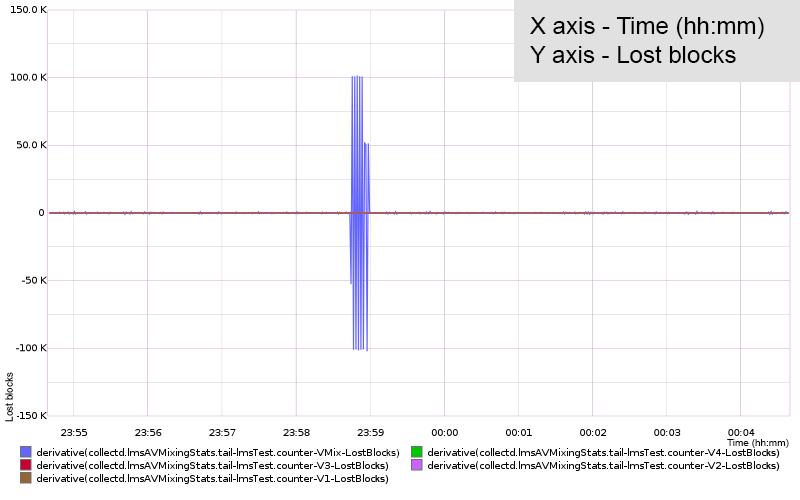
\includegraphics[width=0.70\textwidth]{./images/testAVMix/AVMixVideoLostBlocsDerivative.png}
\caption{Generic scenario - derivative function of the video path accumulated lost blocks}
\label{F:gsvpalbd}
\end{center}
\end{figure}

It is important to note that in Figure \ref{F:gsvpalbd} (also in previous Chapter \ref{H:platformDeploymentAndDemonstrations} figures) there is some noisy data which are caused by the use of working static files to simulate live audio-video streaming. This means that when a file ends some seconds of discontinuity are noticed.

Related to the LMS framework development plan, it is demonstrated that the selected third party libraries are suitable to continue being used (i.e.: Live555, LibAV/ffmpeg, x264 and OpenCV, among others) because they achieve an acceptable performance (i.e: the results show that the filters where they are implemented do not add critical processing time). And, regarding behaviour debugging tools for the LMS, it is possible to know which filters are critical or which should be improved thanks to the implemented metrics gathering system (i.e.: developers are now able to know how many time a filter takes to process a frame).

It is also important to remark that thanks to the developments done related to metrics gathering and the tools deployed around the LMS, it is easier to detect issues in the future. For example, Figure \ref{SF:S5} showed that the processing time for the audio "receiver to mixer" path was not working properly due to not cleaning up the queues when the source is sending in a pseudo-live mode (i.e.: a loop, a periodic reinitialization of the audio stream).

Finally, note that the generic scenario, which performs audio and video mixing from multiple inputs, demonstrates that the video pipeline introduces around 80 milliseconds of processing time. However, most of this delay is due to the encoder (i.e.: x264 library) and the mixer (i.e.: OpenCV library) filters (the "mixer to trasmitter" path).

\section{Collectd and Graphite}

The selection of these tools for the monitoring layer is a good choice when the goal is to have a lightweight and highly configurable system. 

A critical issue about clustering such tools (i.e.: Collectd clustering) is how its bandwidth usage may affect the whole system performance. Figures \ref{F:tscbu} and \ref{F:avmscbu}, which are a filtered whireshark capture of the UDP stream bandwidth usage from the Collectd client to the Collectd and Graphite server, demonstrates that despite the huge amount of parameters to be sent, the communication protocol is lightweight and is not an issue that the system might suffer from. In the worst case (i.e.: generic scenario) the bandwidth usage average is below 70 kbps.

\begin{figure}[!htb]
\begin{center}
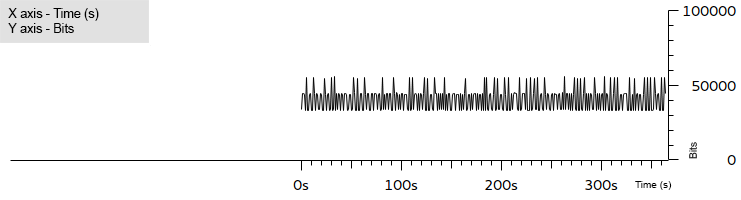
\includegraphics[width=0.70\textwidth]{./images/testStats/testStatsDocker/collectdBWbits.png}
\caption{Transcoder scenario - Collectd bandwidth usage (bits per second)}
\label{F:tscbu}
\end{center}
\end{figure}

\begin{figure}[!htb]
\begin{center}
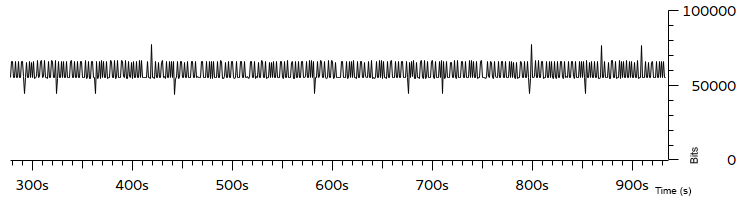
\includegraphics[width=0.70\textwidth]{./images/testAVMix/collectdBWbits.png}
\caption{Audio and video mixer scenario - Collectd bandwidth usage (bits per second)}
\label{F:avmscbu}
\end{center}
\end{figure}

\vbox{Regarding the Graphite tool it is important to remark its huge amount of features to present and treat the metrics, which help to carry out proper graphical data mining. It is also remarkable its compatibility with external tools in order to implement alarm systems or near real-time actuators over the system which is being monitored. This fact is a key point in order to implement a cloud real-time media production platform service.}

Regarding the amount of data to be stored, thanks to the RRD, once the periodicity and granularity of time points are defined the required storage capacity is known and remains constant in time. This is a key point that ensure the system performance will not be affected because of the HDD usage.

There is a last point to highlight about Graphite, which is its capability to offer graphics and specific data through its HTTP API. This means that specific applications are able to display data performance, in many ways, in near real-time.

\section{Docker}

Regarding this virtualization system implemented. Docker has demonstrated to be a proper tool to encapsulate each one of the required pieces of the platform in order to develop, test, distribute and play with them.

Moreover, Docker offers to this platform prototype to become a multiplatform tool, which means that any piece of this prototype can be executed in any OS which Docker gives support (i.e.: currently supported OS are Linux/Unix, MacOSX and Windows).

Thanks to this tool, the global platform becomes fast to scale due to its fast start-up, restart and shut-down times. And this is also due to its ease to quickly replicate any containerized application or service, if required. 

Despite its strengths, it is not still a mature technology (the company behind, called dotCloud, and Docker project itself were born in 2013) but it is evolving really fast. This is demonstrated by the high growth that its community is taking place year by year. 

An area to be improved, which should be solved by Docker itself or through external solutions, are security issues. This is mainly due to the fact that when running a containerized LMS this container does not completely isolate LMS from the security considerations of running it directly on the host; in fact it adds more security vulnerabilities. The most important of these is that the Docker daemon's API does not require any kind of authentication. It is important to make sure that there is a good firewall configured to isolate the host machine from outside the host, or it might be prone to external attacks. Docker's bridged networking as well as mounted file system support allows for possible security holes into and out of the container itself, but this might happen also with traditional virtualization. Of course, the topic of container security is an extensive subject, but it is an issue to be strongly considered when creating a container in order to guarantee the security of Docker (and LXC).

Despite the aforementioned issues, Docker offers other interesting solutions like direct hardware access (i.e.: non specific GPU drivers nor emulator are required) and security at infrastructure management level (i.e.: fast replication and relocation of the containers when specific containers are running with troubles like external network attacks to the service). 

\section{Platform}

The platform developed and tested in this project can be considered the tip of the iceberg of a cloud real-time and live media production platform. Therefore, the outcomes of this thesis are specific tools/solutions which are suitable to be used together or separated, which might lead to future implementations of new specific and higher level tools (e.g.: dynamic platform configuration through browser application). 

We can conclude the main goals of this project has been achieved and are ready to be used.

In order to comply the premise to be as open as possible, a web site of the LMS framework has been published  at \href{http://livemediastreamer.i2cat.net}{http://livemediastreamer.i2cat.net} in order to start building a community of users and developers.

\section{Next steps}

New user requirements should be gathered, guiding new developments, but assuring the requirement to offer a set of tools as much configurable as possible.

In order to improve some filter steps a possibility is to work over GPGPUs (General Purpose Graphic Processing Units). In this case, OpenCV is already offering specific APIs to work over CUDA. Such implementations could lead to develop UHD video pipelines.

Regarding the network side, and thanks to the APIs implemented, it seems feasible to analyse possibilities to deploy these thesis tools within SDN environments, which should improve management and resource optimization.

Other possible future lines could be related to implement new codec and new media formats in order to keep up with the codec market.

In order to improve streaming robustness, a FEC implementation is also a point to explore but keeping in mind to optimize the bandwidth and delay (i.e.: processing time) overheads. There are specific and proprietary solutions but we propose to implement the standard described in RFC 5109 (RTP Payload Format for Generic Forward Error Correction). It is also important to  support specific synchronization mechanisms (in order to assure accurate streams synchronizations), such as PTP (Precision Time Protocol - IEEE 1588-2008 standard), which is a protocol used to synchronize clocks throughout a computer network.

\vbox{Finally, in order to offer a complete set of tools for private media production use cases and to maintain specific license agreements (i.e.: IPR - Intellectual Property Rights) it is also proposed to implement DRM (Digital Rights Management) technology.}
